\documentclass[11pt]{jarticle}
\usepackage[a4paper,hmargin=20mm,vmargin=15pt]{geometry}
\usepackage{amsmath}
\usepackage{amsthm}
\usepackage{amssymb}
\usepackage[dvipdfmx]{graphicx}
\usepackage{float}
\pagestyle{plain}
\begin{document}
\title{}
\date{}
\maketitle
\paragraph{問題.1}
(3) $z=k$と置く. $S$の存在範囲から$k$が$0\leq k \leq \frac{1}{2}$
の時の断面積を積分すればよい. 各$k$の断面積を$S_k$と置き, また次の断面図のとおり$\theta$を置く.
\begin{figure}[H]
\centering
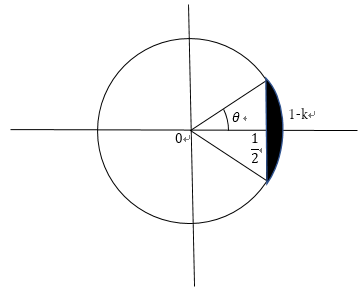
\includegraphics[width=5cm]{fig.png}
\end{figure}
すると$\cos\theta=\frac{1}{2(1-k)}$ ($0 \leq \theta < \frac{\pi}{2}$ )が成立する. 
\begin{align*}
-\sin \theta d\theta& =\frac{1}{2(1-k)^2}dk\\
 S_k & = \frac{1}{2}(1-k)^2 2\theta-\frac{1}{2}(1-k)^2\sin2\theta\\
  &=(1-k)^2\theta-\frac{1}{2}(1-k)^2\sin2\theta\\
\end{align*}
であって$k$が$0$から$\frac{1}{2}$まで動くとき$\theta$は$\frac{\pi}{3}$から$0$まで単調に動くので

\begin{align*}
  \int_0^\frac{1}{2} S_k dk&=\int_\frac{\pi}{3}^0 -\frac{\theta\sin\theta}{8\cos^4\theta}+\frac{\sin\theta\sin 2\theta}{16\cos^4\theta} d\theta\\
                                  &=\int_\frac{\pi}{3}^0 -\frac{\theta\sin\theta}{8\cos^4\theta}+\frac{\sin^2\theta}{8\cos^3\theta} d\theta\\
  &=\int_\frac{\pi}{3}^0\frac{\theta}{24}(\cos^{-3}\theta)'+\frac{1}{8\cos^3\theta}-\frac{1}{8\cos\theta} d\theta\\
  &=\frac{1}{24}\Bigl[\frac{\theta}{\cos^3\theta}\Bigl]_\frac{\pi}{3}^{0}-\frac{1}{24}\int_\frac{\pi}{3}^0\frac{1}{\cos^3\theta}+\frac{1}{8}\int_\frac{\pi}{3}^0\frac{1}{\cos^3\theta}-\frac{1}{8}\int_\frac{\pi}{3}^0\frac{1}{\cos\theta}\\
  &=\frac{\pi}{9}-\frac{1}{12}I_3-\frac{1}{8}I_1\\
  &=\frac{\pi}{9}-\frac{1}{12}\Bigl(\frac{\sqrt3}{2}+\frac{1}{2}I_1\Bigl)-\frac{1}{8}I_1
\end{align*}
\end{document} 